\documentclass[11pt]{article}
%\usepackage{amsfonts}
\usepackage{amsmath}
\usepackage{fancybox}%,times}
\usepackage{graphicx,psfrag,epsf}
%\usepackage{amsmath}
\usepackage{enumerate}
\usepackage{graphicx,psfrag}
\usepackage{multirow}
\usepackage{epsfig}
\usepackage[svgnames]{xcolor}
%\usepackage{rotating}
\usepackage{subfigure}
\usepackage{theorem}
\usepackage{natbib,psfrag}
\usepackage{tikz}
\usepackage{xcolor}
\usepackage{kotex}
\newcommand{\blind}{0}
\usepackage{graphicx}
\usepackage{listings}


%\documentclass[a4paper,12pt]{article}
\usepackage[utf8]{inputenc}

% Default fixed font does not support bold face
\DeclareFixedFont{\ttb}{T1}{txtt}{bx}{n}{12} % for bold
\DeclareFixedFont{\ttm}{T1}{txtt}{m}{n}{12}  % for normal

% Custom colors
\usepackage{color}
\definecolor{deepblue}{rgb}{0,0,0.5}
\definecolor{deepred}{rgb}{0.6,0,0}
\definecolor{deepgreen}{rgb}{0,0.5,0}

\usepackage{listings}
\DeclareGraphicsExtensions{.pdf,.png,.jpg}

\addtolength{\oddsidemargin}{-.75in}%
\addtolength{\evensidemargin}{-.75in}%
\addtolength{\textwidth}{1.5in}%
\addtolength{\textheight}{1.3in}%
%\addtolength{\topmargin}{-.6in}%
\addtolength{\topmargin}{-.8in}%

%\theoremstyle{break}
\newtheorem{The}{Theorem}
\newtheorem{Def}{Definition}
\newtheorem{Pro}{Proposition}
\newtheorem{Lem}{Lemma}
\newtheorem{Cor}{Corollary}
\newtheorem{asp}{Assumption}


\renewcommand{\thefootnote}{\arabic{footnote}}
%\renewcommand{\thefootnote}{\alph{footnote}}
%\renewcommand{\thefootnote}{\roman{footnote}}
%\renewcommand{\thefootnote}{\fnsymbol{footnote}}

\begin{document}
	
	
	%\bibliographystyle{natbib}
	
	\newcommand{\Ito}{$It\hat{o}$'$s~Lemma$}
	
	\newcommand\ind{\stackrel{\rm ind}{\sim}}
	\newcommand\iid{\stackrel{\rm iid}{\sim}}
	\renewcommand\c{\mathbf{c}}
	\newcommand\y{\mathbf{y}}
	\newcommand\z{\mathbf{z}}
	\renewcommand\P{\mathbf{P}}
	\newcommand\W{\mathbf{W}}
	\newcommand\X{\mathbf{X}}
	\newcommand\Y{\mathbf{Y}}
	\newcommand\Z{\mathbf{Z}}
	\newcommand\J{{\cal J}}
	\newcommand\B{{\cal B}}
	\newcommand\K{{\cal K}}
	\newcommand\N{{\rm N}}
	\newcommand\bs{\boldsymbol}
	\newcommand\bth{\bs\theta}
	\newcommand\bbe{\bs\beta}
	\renewcommand\*{^\star}
	\newcommand{\notimplies}{%
		\mathrel{{\ooalign{\hidewidth$\not\phantom{=}$\hidewidth\cr$\implies$}}}}
	
	\def\spacingset#1{\renewcommand{\baselinestretch}%
		{#1}\small\normalsize} \spacingset{1}
	
	
	%%%%%%%%%%%%%%%%%%%%%%%%%%%%%%%%%%%%%%%%%%%%%%%%%%%%%%%%%%%%%%%%%%%%%%%%%%%%%%
	
	\bigskip
	\bigskip
	\bigskip
	\begin{center}
		{\LARGE\bf 2019 Oct. 17 }
	\end{center}
	\begin{center}
		2018321084 Juyoung Ahn
	\end{center}
	\medskip
	
	%\begin{abstract}
	%\end{abstract}
	
	%\noindent%
	%{\it Key Words:}  AECM algorithm; Astrophysical data analysis;
	%ECME algorithm; Incompatible Gibbs sampler; Marginal data
	%augmentation; Multiple imputation; Spectral analysis
	
	\spacingset{1.45}
	\section{Changing point model}
	\subsection{likelihood and prior}
	\begin{align*}
	\beta_t &\iid \begin{cases}
	 Poisson(\lambda)\;\; t= 1, \dots ,k \\
	 Poisson(\phi) \;\; t= k+1, \dots ,T
	\end{cases}\\
	\lambda &\sim Gamma(a,b)\\
	\phi &\sim Gamma(c,d)\\
	k &\sim unif\{1, T\}
	\end{align*}
	\subsection{Gibbs sampler}
	\begin{align*}
	\lambda | \phi,k,\beta &\sim Gamma(a + \sum_{t=1}^{k}\beta_t, k +b)\\
	\phi | \lambda,k,\beta &\sim Gamma(c + \sum_{t=k+1}^{T}\beta_t, T-k+d)\\
	p(k | \lambda,\phi,\beta) &= \frac{\exp(k(\phi- \lambda)+ \log(\lambda/\phi)\sum_{i=1}^{k}\beta_t)}{\sum_{t=1}^{T}\exp(k(\phi- \lambda)+ \log(\lambda/\phi)\sum_{t=1}^{k}\beta_t)}
	\end{align*}
	\subsection{Variational Bayes}
	\begin{align*}
	q_1^*(\lambda)  &\sim Gamma(a + \sum_{t=1}^{E_{q_3^*}[k]}\beta_t, E_{q_3^*}[k] +b)\\
	q_2^*(\phi) &\sim Gamma(c + \sum_{t=E_{q_3^*}[k]+1}^{T}\beta_t, T-E_{q_3^*}[k]+d)\\
	q^*(k) &= \frac{\exp(k(E_{q_2^*}[\phi]- E_{q_1^*}[\lambda])+ \log(E_{q_1^*}[\log(\lambda)]- E_{q_2^*}[\log(\phi)])\sum_{t=1}^{k}\beta_t)}{\sum_{k=1}^{T}\exp(k(E_{q_2^*}[\phi]- E_{q_1^*}[\lambda])+ \log(E_{q_1^*}[\log(\lambda)]- E_{q_2^*}[\log(\phi)])\sum_{t=1}^{k}\beta_t)}
	\end{align*}
	We can use
	\begin{align*}
	X \sim Gamma(\alpha,\beta)\\
	E[\log X] = -\log\beta +\psi(\alpha)
	\end{align*}
	where $\psi$ means digamma function
	
	\section{Simulation}
	Make simulation data from
	\begin{align*}
	\beta_t &\iid \begin{cases}
	Poisson(1)\;\; t= 1, \dots ,30 \\
	Poisson(3) \;\; t= 31, \dots ,100
	\end{cases}
	\end{align*}
	
	\begin{figure}[h]
		\centering
		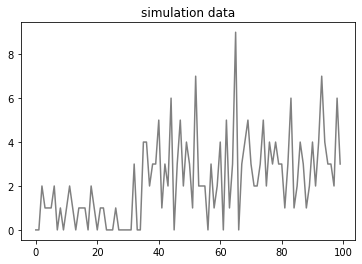
\includegraphics[width=0.7\linewidth]{simuldata}
		\caption{Simulated data time series plot}
		\label{fig:simuldata}
	\end{figure}
	\subsection{Gibbs}
	Prior and initial value are
	\begin{align*}
	a = 4;\;
	b = 1;\;
	c = 1;\;
	d = 2\\
	\phi = 1
	\end{align*}
	
	\begin{figure}
		\centering
		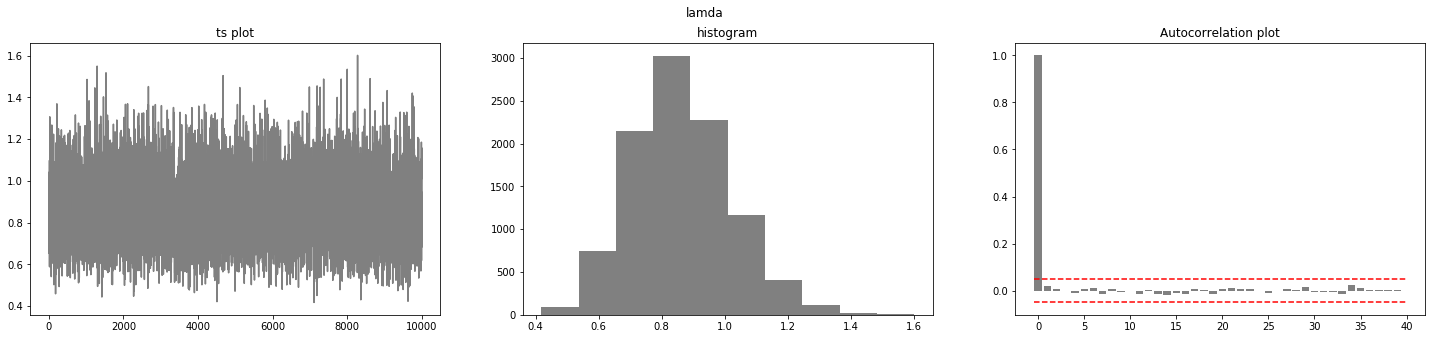
\includegraphics[width=1\linewidth]{gibbslam}
		\caption{Gibbs sampling for $\lambda$}
		\label{fig:gibbslam}
	\end{figure}
	\begin{figure}
		\centering
		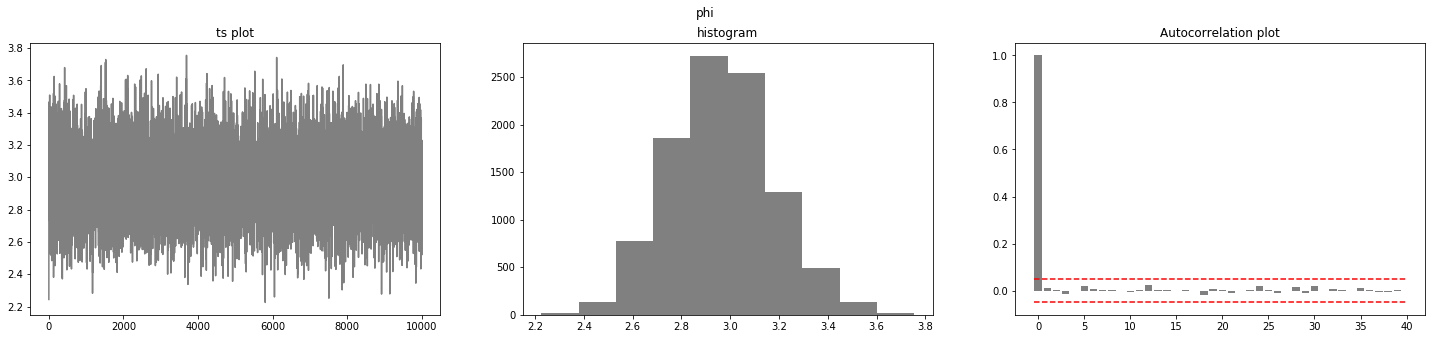
\includegraphics[width=1\linewidth]{gibbspi}
		\caption{Gibbs sampling for $\phi$}
		\label{fig:gibbspi}
	\end{figure}
	
	\begin{figure}
		\centering
		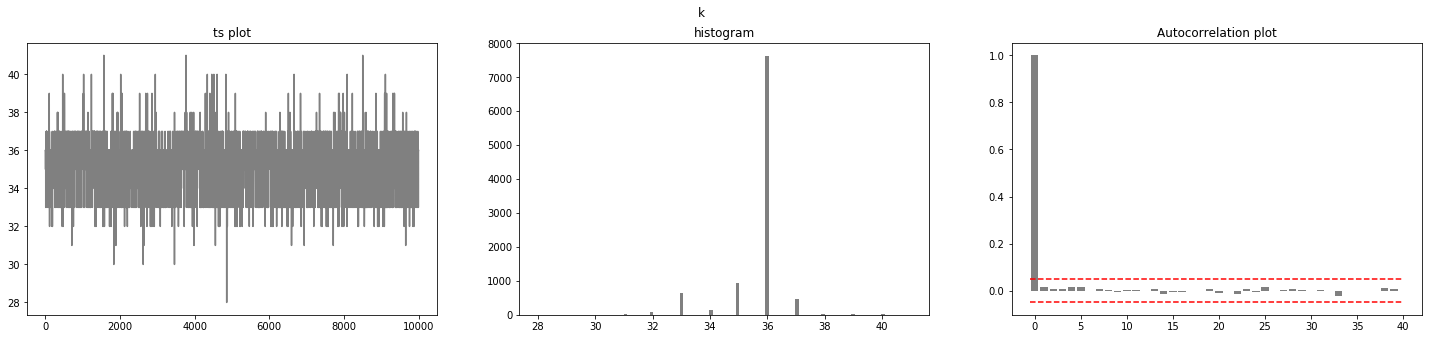
\includegraphics[width=1\linewidth]{gibbsk}
		\caption{Gibbs sampling for $k$}
		\label{fig:gibbsk}
	\end{figure}
	\subsection{VI}
	Prior and initial value are
	\begin{align*}
	a = 4;\;
	b = 1;\;
	c = 1;\;
	d = 2\\
	k = 1
	\end{align*}
	Variational distribution is
	\begin{align*}
	q_1^*(\lambda)  &\sim Gamma(32.0, 36.72)\\
	q_2^*(\phi) &\sim Gamma(196.0, 66.28)
	\end{align*}
	and $q_3^*$ is
	\begin{figure} [h]
		\centering
		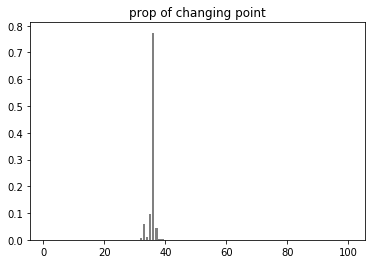
\includegraphics[width=0.7\linewidth]{vi}
		\caption{Variational distribution of $q_3^*$}
		\label{fig:vi}
	\end{figure}
	\begin{align*}
	E_{q_3}^*[k] = 35.72
	\end{align*}

\end{document}